\documentclass[10pt,a4paper]{article}

\usepackage[margin=0.7in,top=0.65in,bottom=0.7in]{geometry}
\usepackage{amsmath,amssymb}
\usepackage{booktabs}
\usepackage[expansion=false]{microtype}
\usepackage{enumitem}
\usepackage{xurl}
\usepackage[hidelinks]{hyperref}
\usepackage{pgfplots}
\pgfplotsset{compat=1.16}
\usepackage{caption}
\captionsetup{font=small,labelfont=bf}
\usepackage{graphicx}

\usepackage{titlesec}
\titlespacing*{\section}{0pt}{5pt}{2pt}
\titlespacing*{\subsection}{0pt}{4pt}{1pt}
\titlespacing*{\paragraph}{0pt}{3pt}{6pt}
\titleformat*{\section}{\large\bfseries}
\titleformat*{\subsection}{\normalsize\bfseries}
\setlength{\textfloatsep}{6pt}
\setlength{\intextsep}{6pt}
\setlength{\abovecaptionskip}{3pt}
\setlength{\belowcaptionskip}{2pt}
\setlist{nosep,leftmargin=*}
\setlength{\parskip}{1pt}
\setlength{\parindent}{0pt}
\raggedbottom
\setlength{\emergencystretch}{2em}

\begin{document}

% ---------- Title Page ----------
\begin{titlepage}
\centering
\vspace*{1.2cm}

\IfFileExists{iitd.png}{{\includegraphics[width=4.2cm]{iitd.png}}}{}

\vspace{1.0cm}

{\huge\scshape Indian Institute of Technology Delhi\par}

\vspace{0.4cm}

{\Large COL764: Information Retrieval and Web Search\par}

\vspace{2.2cm}

{\rule{0.85\textwidth}{0.8pt}\par}
\vspace{0.6cm}
{\LARGE\bfseries Assignment 2: Relevance Feedback and Reranking\par}
\vspace{0.6cm}
{\rule{0.85\textwidth}{0.8pt}\par}

\vspace{2.5cm}

\begin{minipage}{0.45\textwidth}
\centering
{\Large\bfseries Submitted by}\par
\vspace{0.25cm}
{\Large Aditya Anand\par}
{\Large 2023CS50284\par}
\end{minipage}%
\begin{minipage}{0.45\textwidth}
\centering
{\Large\bfseries Instructor}\par
\vspace{0.25cm}
{\Large Prof.\ Srikanta Bedathur\par}
\end{minipage}

\vfill

{\Large \today\par}

\vspace{1cm}

\end{titlepage}

% ---------- Report content begins ----------
\newpage

\section{Algorithms}

Tokens are lowercase alphanumeric words. Dotted single letters are joined into acronyms. Query stopwords are removed and tokens are Porter-stemmed. Three unigram document models are implemented.

\begin{align*}
P_{\mathrm{Dir}}(w\mid D) &= \frac{\mathrm{tf}(w,D) + \mu\, P(w\mid C)}{|D| + \mu}, &
P_{\mathrm{JM}}(w\mid D) &= (1-\lambda_{\mathrm{JM}})\frac{\mathrm{tf}(w,D)}{|D|} + \lambda_{\mathrm{JM}} P(w\mid C), \\
P_{\mathrm{SPUD}}(w\mid D) &= \frac{|V_D|\cdot \mathrm{tf}(w,D)/|D| + \omega\, P_{\mathrm{df}}(w)}{|V_D| + \omega}.
\end{align*}

$P(w\mid C)$ is the collection frequency. $P_{\mathrm{df}}$ is the document frequency, normalised over the vocabulary. $|V_D|$ is the number of distinct terms in $D$. The submitted model is SPUD with $\omega = 800$, plus a Dirichlet model of the first 20 tokens (weight $0.1$, $\mu = 60$) and sequential dependence. Ordered adjacent bigrams have weight $0.05$ and unordered pairs in a window of 9 have weight $0.1$, both Dirichlet-smoothed with $\mu = 450$. The Dirichlet and Jelinek--Mercer baselines are plain unigrams. Their proximity and lead weights are zero.

The relevance model uses only the supplied seed. Unknown ids are ignored. For the submitted model I sharpen $P(D\mid Q)$ with $\beta = 40$, drop a seed document that covers less than a quarter of the query and keep at most five documents. RM1 and RM2 follow Lavrenko and Croft. Inside that estimate $P(w\mid D)$ is Dirichlet with $\mu = 100$, and that smoother is only used to build $P(w\mid R)$. Candidates are still scored with the Track~A model.

\begin{align*}
P_{\mathrm{RM1}}(w\mid R) &= \sum_{D \in \mathrm{seed}} P(w\mid D)\, P(D\mid Q), &
P_{\mathrm{RM2}}(w\mid R) &\propto P(w) \prod_{q \in Q} \sum_{D} P(q\mid D)\, P(D\mid w).
\end{align*}

A term is dropped unless it occurs in at least a fifth of the seed (\texttt{support\_frac}${=}0.2$). Query terms are kept. Inverse document frequency only decides which terms survive. The distribution is then cut to 80 terms and renormalised. RM1 ranks by $\sum_w P(w\mid R)\log P(w\mid D)$. RM2 uses the same score with $P_{\mathrm{RM2}}$. RM3 puts weight $\lambda$ back on the query. The baselines use the usual interpolation. On the submitted model I leave the Track~A score as it is and center the expansion over the pool, so the two scores can be added:
\[
S(D) = \lambda\, S_A(D) + (1-\lambda)\,\frac{E(D) - \mathrm{mean}\, E}{12},
\qquad
E(D) = \sum_w P_{\mathrm{RM1}}(w\mid R)\, \log P_{\mathrm{SPUD}}(w\mid D).
\]
$\lambda = 0$ is pure RM1. $\lambda = 1$ returns the Track~A ranking and the Track~A scores, so turning the expansion off does not change \texttt{score\_candidates()}.

\section{How this model was reached}

I checked Dirichlet, Jelinek--Mercer, RM1, RM2 and RM3 on a five-document hand example before any tuning. On the dev set Dirichlet ($\mu{=}360$) scores 0.6076 and Jelinek--Mercer ($\lambda_{\mathrm{JM}}{=}0.35$) scores 0.5434. Lengths vary a lot and only Dirichlet scales the smoothing with length. SPUD, the lead field and proximity, still as query likelihood, take Track~A from 0.6076 to 0.6521. Each hidden upload below is the five numbers the leaderboard prints.

\begin{center}
\scriptsize
\begin{tabular}{lccccc}
\toprule
Hidden upload & A nDCG & A MAP & B nDCG & C1 & C2 \\
\midrule
Early single model & 0.53295 & 0.45387 & 0.53373 & 1.00000 & --- \\
Two parameter sets, A and B separate & 0.53821 & 0.45985 & 0.53289 & 1.00000 & 0.78241 \\
One model, but B below A & 0.53820 & 0.46070 & 0.53783 & 1.00000 & 0.99927 \\
Translation model on query terms & 0.53558 & --- & --- & --- & --- \\
Submitted: one model, B above A & 0.53809 & 0.46063 & 0.53814 & 1.00000 & 0.99854 \\
\bottomrule
\end{tabular}
\end{center}

That first upload was one language model and the retriever was weak. Separate parameters for Track~A and Track~B raised Track~A to 0.53821 and dropped Track~B to 0.53289. C1 stayed at 1.00000 and C2 fell to 0.78241. The later clarification does not allow that split so I removed it. One shared model, with Track~B still below Track~A, left C2 at 0.99927. A translation model on the query terms then cut Track~A from 0.53809 to 0.53558 and I took it out. The submitted run is RM3 at $\lambda{=}0.9$ on SPUD. Track~B is 0.00005 above Track~A (C1 1.00000, C2 0.99854).

\section{Dev-set results}

Dev numbers are nDCG@10 from \texttt{harness/run\_harness.py} on the released full dev set. Noise is one deterministic draw per query from \texttt{noise\_injection.py}, so the same seeds are compared across $\lambda$. Retention is that noisy nDCG divided by the same row's clean nDCG.

\begin{center}
\footnotesize
\begin{tabular}{llcccc}
\toprule
Model & Feedback & Clean & 25\% & 50\% & Retention@50 \\
\midrule
Competition, A${=}0.6521$ & RM1 & 0.6703 & 0.6592 & 0.6327 & 0.944 \\
 & RM2 & 0.6492 & 0.6344 & 0.6266 & 0.965 \\
 & RM3, $\lambda{=}0.9$ & \textbf{0.6534} & \textbf{0.6533} & \textbf{0.6546} & \textbf{1.002} \\
\midrule
Dirichlet, A${=}0.6076$ & RM1 & 0.6262 & 0.6139 & 0.6131 & 0.979 \\
$\mu{=}360$, 2 docs, 30 terms & RM2 & 0.6166 & 0.6154 & 0.5943 & 0.964 \\
 & RM3, $\lambda{=}0.45$ & 0.6582 & 0.6473 & 0.6407 & 0.973 \\
\midrule
Jelinek--Mercer, A${=}0.5434$ & RM1 & 0.5925 & 0.5823 & 0.5669 & 0.957 \\
$\lambda_{\mathrm{JM}}{=}0.35$, 7 docs, 100 terms & RM2 & 0.5505 & 0.5487 & 0.5351 & 0.972 \\
 & RM3, $\lambda{=}0.3$ & 0.6030 & 0.5925 & 0.5890 & 0.977 \\
\bottomrule
\end{tabular}
\end{center}

On the competition model RM1 is best on a clean seed and worst under noise: $0.6327/0.6703 = 0.944$. RM2 is below RM1 on every model. Its retention is still higher than RM1 on the competition model (0.965 against 0.944) and on Jelinek--Mercer (0.972 against 0.957), and lower only on Dirichlet (0.964 against 0.979), so the problem is the estimate, not extra fragility. On the competition model, RM3 is the only row above Track~A (0.6521) at 0\%, 25\% and 50\% noise. Several Dirichlet and Jelinek--Mercer rows are also above their own Track~A. Dirichlet RM3 goes from 0.6076 to 0.6582 clean (retention 0.973) because that first stage still has more to fix. On the submitted model the move is from 0.6521 to 0.6534. On that one draw the 50\% score is slightly above the clean score.

\begin{figure}[ht]
\centering
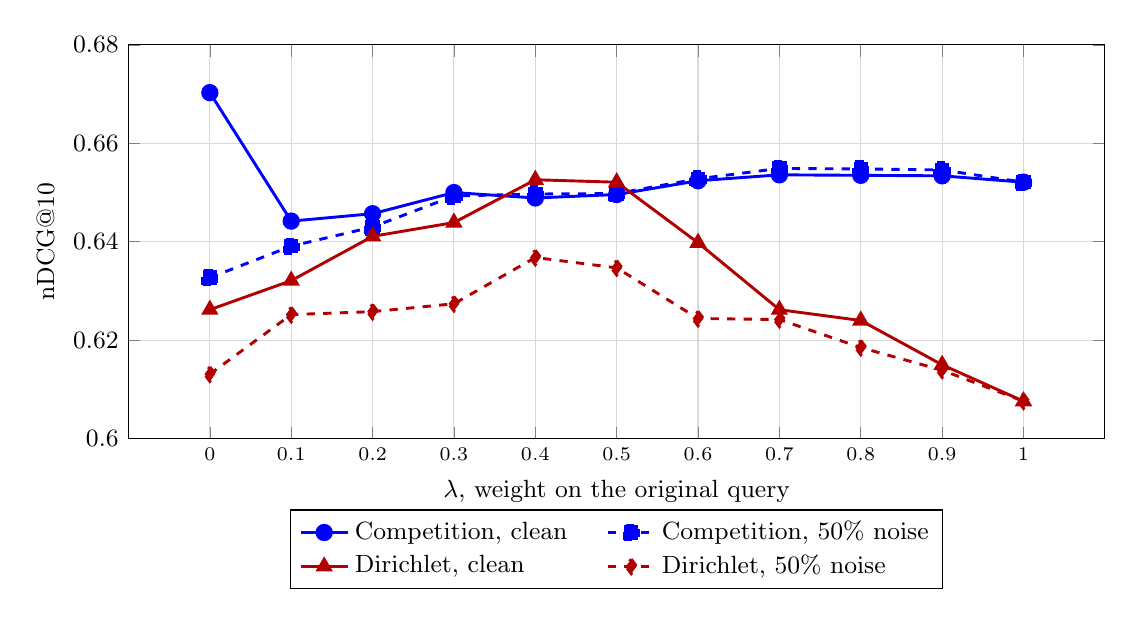
\begin{tikzpicture}
\begin{axis}[
  width=12.4cm, height=5.0cm, scale only axis,
  xlabel={$\lambda$, weight on the original query},
  ylabel={nDCG@10},
  ymin=0.60, ymax=0.68,
  ytick={0.60,0.62,0.64,0.66,0.68},
  xtick={0,0.1,0.2,0.3,0.4,0.5,0.6,0.7,0.8,0.9,1},
  xticklabel style={font=\scriptsize},
  tick label style={font=\small},
  label style={font=\small},
  axis line style={black},
  grid=both,
  major grid style={gray!30},
  legend style={font=\small, draw=black, fill=white,
                at={(0.5,-0.18)}, anchor=north, legend columns=2,
                /tikz/every even column/.append style={column sep=1.2em}},
  legend cell align=left,
  every axis plot/.append style={line width=1.05pt, mark size=2.6pt},
]
\addplot[color=blue, mark=*] coordinates {(0,0.6703) (0.1,0.6442) (0.2,0.6457) (0.3,0.6500) (0.4,0.6489) (0.5,0.6496) (0.6,0.6524) (0.7,0.6536) (0.8,0.6535) (0.9,0.6534) (1,0.6521)};
\addlegendentry{Competition, clean}
\addplot[color=blue, dashed, mark=square*] coordinates {(0,0.6327) (0.1,0.6391) (0.2,0.6430) (0.3,0.6493) (0.4,0.6497) (0.5,0.6498) (0.6,0.6528) (0.7,0.6549) (0.8,0.6548) (0.9,0.6546) (1,0.6521)};
\addlegendentry{Competition, 50\% noise}
\addplot[color=red!70!black, mark=triangle*] coordinates {(0,0.6262) (0.1,0.6321) (0.2,0.6411) (0.3,0.6439) (0.4,0.6526) (0.5,0.6521) (0.6,0.6398) (0.7,0.6262) (0.8,0.6240) (0.9,0.6150) (1,0.6076)};
\addlegendentry{Dirichlet, clean}
\addplot[color=red!70!black, dashed, mark=diamond*] coordinates {(0,0.6131) (0.1,0.6252) (0.2,0.6258) (0.3,0.6274) (0.4,0.6368) (0.5,0.6347) (0.6,0.6244) (0.7,0.6242) (0.8,0.6185) (0.9,0.6139) (1,0.6076)};
\addlegendentry{Dirichlet, 50\% noise}
\end{axis}
\end{tikzpicture}
\caption{nDCG@10 against $\lambda$ on the TREC-COVID dev set, in steps of $0.1$. Solid lines are a clean seed. Dashed lines are 50\% practice noise. $\lambda = 0$ is pure RM1. $\lambda = 1$ is Track~A. The submitted point is $\lambda = 0.9$.}
\end{figure}

\begin{center}
\small
\begin{tabular}{lcccc}
\toprule
$\lambda$ & Comp.\ clean & Comp.\ 50\% & Dir.\ clean & Dir.\ 50\% \\
\midrule
0.0 & 0.6703 & 0.6327 & 0.6262 & 0.6131 \\
0.1 & 0.6442 & 0.6391 & 0.6321 & 0.6252 \\
0.2 & 0.6457 & 0.6430 & 0.6411 & 0.6258 \\
0.3 & 0.6500 & 0.6493 & 0.6439 & 0.6274 \\
0.4 & 0.6489 & 0.6497 & 0.6526 & 0.6368 \\
0.5 & 0.6496 & 0.6498 & 0.6521 & 0.6347 \\
0.6 & 0.6524 & 0.6528 & 0.6398 & 0.6244 \\
0.7 & 0.6536 & 0.6549 & 0.6262 & 0.6242 \\
0.8 & 0.6535 & 0.6548 & 0.6240 & 0.6185 \\
\textbf{0.9} & \textbf{0.6534} & \textbf{0.6546} & 0.6150 & 0.6139 \\
1.0 & 0.6521 & 0.6521 & 0.6076 & 0.6076 \\
\bottomrule
\end{tabular}
\end{center}

The 50\% column above is one noise seed. Over ten seeds on the competition model, $\lambda{=}0.9$ has mean nDCG@10 $0.6537$ (standard deviation $0.0006$) and mean retention $1.000$ (standard deviation $0.0009$). $\lambda{=}0$ has mean nDCG $0.6466$ (standard deviation $0.014$) and mean retention $0.965$ (standard deviation $0.020$). Below about $\lambda = 0.4$ the clean curve is above the noisy one: expansion helps a clean seed and hurts a noisy one. From $0.6$ to $1.0$ the two competition curves stay within $0.003$. On this grid the flat part peaks at $\lambda{=}0.7$ (0.6536 clean, 0.6549 at 50\%), which is $0.0002$ above $\lambda{=}0.9$. Dirichlet's 50\% curve peaks at $0.4$ and then falls. Its tuned point, $\lambda{=}0.45$, is the 0.6582 row. That clean score beats the submitted RM3, but Track~A is 0.6076 against 0.6521 and retention is 0.973 against 1.002.

\section{Submitted model on every local collection}

The same competition RM3, $\lambda{=}0.9$, on every collection that has a candidate file. Noise is the same practice recipe, one draw per query. Retention is the 50\% score divided by the clean score.

\begin{center}
\footnotesize
\begin{tabular}{lrrrrrr}
\toprule
Collection & \#q & Track~A & Clean & 25\% & 50\% & Ret. \\
\midrule
Toy & 6 & 0.8716 & 0.8716 & 0.8900 & 0.8716 & 1.000 \\
Cranfield & 225 & 0.2984 & 0.2982 & 0.2982 & 0.2977 & 0.998 \\
CACM & 52 & 0.5018 & 0.5018 & 0.5018 & 0.5018 & 1.000 \\
Vaswani & 93 & 0.4065 & 0.4065 & 0.4058 & 0.4058 & 0.998 \\
SciFact & 300 & 0.7001 & 0.7001 & 0.7001 & 0.7000 & 1.000 \\
NFCorpus & 323 & 0.3195 & 0.3196 & 0.3197 & 0.3198 & 1.001 \\
FiQA & 648 & 0.2673 & 0.2676 & 0.2673 & 0.2676 & 1.000 \\
SciDocs & 1000 & 0.1660 & 0.1658 & 0.1659 & 0.1659 & 1.001 \\
ArguAna & 1406 & 0.3811 & 0.3811 & 0.3811 & 0.3811 & 1.000 \\
Touch\'e-2020 & 49 & 0.4323 & 0.4322 & 0.4322 & 0.4323 & 1.000 \\
Antique & 200 & 0.3837 & 0.3839 & 0.3839 & 0.3839 & 1.000 \\
TREC-COVID dev & 50 & 0.6521 & 0.6534 & 0.6533 & 0.6546 & 1.002 \\
\bottomrule
\end{tabular}
\end{center}

On the ten non-toy collections other than TREC-COVID, nDCG@10 moves by at most $0.0007$ (Cranfield 0.2984 to 0.2977, Vaswani 0.4065 to 0.4058). The toy set is the exception: its 25\% score moves from 0.8716 to 0.8900, because six queries make one swapped document a large swing.

\section{Final $\lambda$ and smoothing}

\begin{center}
\scriptsize
\begin{tabular}{ll}
\toprule
Piece & Submitted setting \\
\midrule
Document model & SPUD, $\omega{=}800$, document-frequency background \\
Lead field & first 20 tokens, weight $0.1$, $\mu{=}60$ \\
Proximity & ordered bigrams $0.05$, window-9 pairs $0.1$, $\mu{=}450$ \\
Feedback model & Dirichlet $\mu{=}100$, at most 5 documents, 80 terms \\
Seed filter & coverage $0.25$, $\beta{=}40$, support $0.2$ \\
RM3 & $\lambda{=}0.9$ \\
\bottomrule
\end{tabular}
\end{center}

The unigram models use Dirichlet smoothing. On the dev set it scores 0.6076 and Jelinek--Mercer scores 0.5434, because document length varies and only Dirichlet scales the prior with length. The submitted model is SPUD with $\omega{=}800$, which keeps that length term and uses a document-frequency background. The lead weight is $0.1$ and the ordered-bigram weight is $0.05$, so neither can override the unigram score. Turning feedback off leaves the Track~A ranking unchanged.

Lower $\lambda$ takes more from the seed. $\lambda{=}0$ is 0.017 higher on a clean run (0.6703 against 0.6534) and about 0.007 lower under the ten noise seeds and mean retention falls from 1.000 to 0.965. At $\lambda{=}0.9$ the expansion is a tenth of the score. The dev change is 0.0013 and the hidden change is 0.00005 (0.53809 to 0.53814; MAP 0.46063; C1 1.00000, C2 0.99854). The noisy-score standard deviation is 0.0006, so the hidden gap sits inside that noise. I kept $0.9$ because retention stays near 1 and nDCG on the ten non-toy collections moves by at most 0.0007. On this grid $\lambda{=}0.7$ is $0.0002$ higher, so the curve is not perfectly flat. I treated the clean score and retention together.


\section{Adversarial set}

The set is five dev queries: 48, 29, 44, 25 and 22. Each list comes from that query's own top-100 pool. Every document is non-relevant or unjudged and each has a high query likelihood, so a model that trusts $P(D\mid Q)$ will treat it as a good seed and push it into the top 10.

I grew each list one document at a time, then tried one swap or deletion when that raised the average drop. The panel was ten of my own setups, each with Porter stemming and with raw tokens: submitted RM3 and RM1, the tuned Dirichlet and Jelinek--Mercer RM3, textbook RM1, RM2 and RM3, RM3 with a uniform document prior, $\lambda = 0.7$, and Dirichlet RM3 with $\mu = 2000$. On that panel the file drops mean nDCG@10 by 0.649 (query 48: 0.702 on 8 documents, 44: 0.671 on 5, 29: 0.657 on 6, 22: 0.625 on 6, 25: 0.589 on 7). The submitted model does not move. Its top 10 is the same on all five queries because $\lambda = 0.9$ leaves little weight on the seed and the coverage filter drops documents that miss most of the query. Typical RM1 and RM3 setups on the panel drop by about 0.6 to 0.9.

\section{Code provenance}

I started from the Assignment~2 code given with the course repository. For the analyzer, Porter stemming and stopword lists I went back to my own Assignment~1 code and carried that over, then kept building the retrieval and feedback on from there. Scoring is C++ and the standard library, loaded with \texttt{ctypes}. No search engine or IR scoring library is used. The stemmer follows Porter's reference implementation with a bounds check on short words. Query stopwords are the NLTK English list. SPUD follows Cummins, Paik and Lv (TOIS, 2015). Dirichlet and Jelinek--Mercer follow Zhai and Lafferty (SIGIR, 2001). RM1--RM3 follow Lavrenko and Croft (SIGIR, 2001).
 
\end{document}
